\documentclass[12pt ]{article} 
\usepackage{amssymb}
\usepackage{amsmath}
\usepackage{geometry}
\geometry{a4paper, total={160mm,240mm}}
\usepackage{graphicx} % Required for inserting images
\usepackage[slovene]{babel}
\usepackage{wrapfig}
\usepackage{comment}
\usepackage{csquotes}

\usepackage[sorting=none]{biblatex}
\addbibresource{viri.bib}
\bibliographystyle{unsrt}
  
\begin{document}
 $~$ 
\vspace{2cm}
\centerline{\bf \huge   Mehka robotika} 
\vspace{1cm} 
\centerline{\huge  Tine Zaletelj}
\vspace{1cm}
\centerline{\large Mentor: prof. dr. Miha Ravnik}
\vspace{1cm}
\centerline{\large Seminar, 3. letnik}
\vspace{1cm}
\centerline{\large Oddelek za fiziko, FMF, UL, 2025/2026}
\vspace{6cm}
  
  \begin{minipage}[c]{0.9\hsize}
  {\bf Povzetek}
  Mehka robotika je veja robotike, ki se ukvarja z roboti iz mehkih materialov. V seminarju bomo spoznali osnove elastomehanike, ki je pomembno fizikalno ozadje. Nato bomo pogledali model človeškega prsta, sledilo pa bo nekaj načinov premikanja mehkih robotov, na primer s pomočjo tlaka in elektrike. Za konec si bomo pogledali še primer mehkega robota-robotsko hobotnico.   
    \end{minipage}

 
 \newpage
  
  
\section{Uvod}
Za razliko od tradicionalnih, trdih robotov, se veja mehke robotike zgleduje po naravi, da naredi zmogljive robote, ki lahko opravljajo več različnih nalog hkrati, njihovo premikanje pa je podobno premikanju živih bitij. Trdi roboti so ponavadi narejeni tako, da lahko opravijo določeno nalogo pod točno določenimi pogoji. Ker so mehki roboti večinoma izdelani iz materialov, katerih elastičnost je primerljiva z elastičnostjo mehkih bioloških sistemov, se lahko premikajo z visokimi stopnjami svobode, na prilagodljiv in varen način komunicirajo z okolico ter se hitro prilagajajo nenadoma spreminjajočim se situacijam\cite{yasa2023overview}.

Mehki roboti so že pokazali svoj potencial za uporabo v vsakdanjem življenju. Na primer, kombinacija mehkih robotskih mehanizmov s klasičnimi roboti se je izkazala za zelo uporabno pri manipulaciji predmetov v industrijskem okolju. Poleg tega so se mehki roboti izkazali tudi v medicini, na primer pri endoskopiji, kirurgiji in dostavi zdravil na točno določena mesta v telesu\cite{yasa2023overview}.
%npr. Robot pobere šrauf, ki je na točno določenem mestu. Če je šrauf postavljen 1cm stran od predvidene lokacije, ga bo klasičen robot zgrešil, mehek robot pa pobral.

Klasični oziroma trdni roboti so narejeni iz trdnih materialov, premikajo pa se s pomočjo elektromotorjev, hidravlike ali pnevmatike. Kontroliranje trdih robotov je dandanes že zelo dobro razvito, ampak je njihovo gibanje pogosto zelo kompleksno. Od tu sledi, da je tudi programiranje takih sistemov zelo zahtevno.

Kljub temu, da je trda robotika zelo uspešna veja robotike, pa ima zaradi svojih lastnosti kar nekaj pomankljivosti:\\
\textbf{Sodelovanje z ljudmi}: Zelo pogosto so zaradi svoje velikosti in trdnosti roboti nevarni za ljudi v svoji bližini. Prav tako pogosto operirajo z nevarnimi orodji ter se hitro premikajo, kar jih naredi še bolj nevarne.\\
\textbf{Preprostost in cena izdelave}: Če želimo, da so trdi roboti natančni, morajo biti izdelani zelo precizno, kar tudi močno dvigne ceno izdelave. V tem pogledu so mehki roboti precej boljši. Namesto robotske roke z veliko motorji in senzorji se mehki roboti zanašajo na elastične lastnosti materiala, iz katerega so sestavljeni. Poleg tega so mehki roboti pogosto sestavljeni iz manj kosov ter nimajo ležajev, v katerih bi se ustvarjalo trenje.\\
\textbf{Ostalo}: Mehki roboti so pogosto lažji in bolj energijsko učinkoviti, poleg tega pa imajo boljše razmerje med težo in maksimalno močjo, ki jo lahko proizvedejo\cite{whitesides2018soft}.

\section{Osnove elastomehanike}
Elastomehanika ima ključno vlogo v mehki robotiki, saj omogoča opis in napoved obnašanja mehkih, deformabilnih materialov, iz katerih so roboti izdelani. Z njeno pomočjo lahko razumemo, kako se strukture iz elastomerov odzivajo na sile, tlake ali električne dražljaje, ter kako se pri tem raztezajo, krivijo ali zvijajo. To je bistveno pri načrtovanju aktuatorjev in prijemal, kjer želimo doseči natančno kontrolirane deformacije brez poškodb materiala. Poleg tega elastomehanski modeli, pogosto nelinearni zaradi velikih deformacij, omogočajo realistično simulacijo gibanja mehkih robotov in optimizacijo njihove oblike ter funkcionalnosti.

Mehki materiali so tisti, ki imajo majhen elastični modul velikostnega reda $10^3-10^7$Pa. Za razliko od togih materialov so mehki materiali zmožni prenesti velike deformacije, poleg tega pa je njihovo obnašanje precej nelinearno, zato linearna teorija deformacij (Hookov zakon) odpove.

Kinematika mehkih robotov se močno razlikuje od kinematike tradicionalnih, trdnih robotov. Zaradi njihove sestave lahko obnašanje mehkih robotov obravnavamo kot obnašanje kontinuuma\cite{rus2015design}.

\subsection{Napetost}
Osno napetost palice $\sigma$ definiramo kot $$\sigma=\frac{F}{A},$$ kjer je $F$ sila, vzporedna z osjo palice, $A$ pa prečni presek palice. V splošnem pa je napetost tenzor $p_{ik},$ ki ga definiramo prek enačbe $$f_i=\frac{\partial p_{ik}}{\partial x_k},$$ kjer je $f_i$ prostorninska gostota sil, $i$ in $k$ pa indeksa, $i,k\in\{x,y,z\}$. Napetostni tenzor ima enote tlaka. Napetostni tenzor je v mehki robotiki ključen zato, ker opisuje kako so sile porazdeljene znotraj deformabilnega materiala v vseh smereh hkrati, kar je bistveno za razumevanje in načrtovanje mehkih struktur.

\subsubsection{Simetričnost napetostnega tenzorja}
Poglejmo si navor na telo.
\begin{align*}
M_i &= \int (\mathbf r \times \mathbf f)_i \, d^3 r
     = \int \epsilon_{ijk} x_j f_k \, d^3 r
     = \int \epsilon_{ijk} x_j \frac{\partial p_{kl}}{\partial x_l} \, d^3 r \\
&= \int \epsilon_{ijk} \frac{\partial (x_j p_{kl})}{\partial x_l} \, d^3 r
   - \int \epsilon_{ijk} \frac{\partial x_j}{\partial x_l} p_{kl} \, d^3 r \\
&= \oint \epsilon_{ijk} x_j p_{kl} \, dA_l
   - \int \epsilon_{ijk} \delta_{jl} p_{kl} \, d^3 r .
\end{align*}
V prvem koraku smo vektorski produkt izrazili z Levi-Citajevim tenzorjem, nato smo gostoto sil zamenjali z divergenco napetostnega tenzorja, nato pa smo uporabili produktno pravilo za odvajanje, da smo dobili dva člena. Prvi člen, ki vsebuje odvod produkta, lahko prek izreka Gauss-Ostrogradskega prepišemo na ploskovni integral, drugi del pa izrazimo z delta-funkcijo.

Ker so sile med deli telesa kontaktne, lahko navor izrazimo kot integral po površini telesa. Od tu sledi, da mora biti drugi integral enak 0: $$0=\epsilon_{ijk}\delta_{jl}p_{kl}=\epsilon_{ijk}p_{kj}=\frac{1}{2}(\epsilon_{ijk}p_{kj}+\epsilon_{ikj}p_{jk})=\frac{1}{2}(\epsilon_{ijk}p_{kj}-\epsilon_{ijk}p_{jk})=\frac{1}{2}\epsilon_{ijk}(p_{kj}-p_{jk}).$$
Najprej smo zaradi Kroneckerjeve delta funkcije zamenjali indeks v napetostnem tenzorju, nato smo izraz zapisali kot vsoto dveh enakih členov, z upoštevanjem antisimetričnosti Levi-Citajevega tenzorja pa smo prišli do končne oblike. Vidimo, da je izraz enak 0 natanko takrat, ko je napetostni tenzor simetričen, oziroma velja $p_{ik}=p_{ki}.$

\subsection{Deformacija}
Za majhne deformacije v eni dimenziji lahko definiramo raztezek kot $$\varepsilon=\frac{\Delta L}{L}.$$ Za materiale, kjer so prisotni veliki raztezki, definiramo raztezno razmerje kot $$\lambda=\frac{L+\Delta L}{L}=1+\varepsilon.$$ V splošnem je deformacija prav tako tenzor, ki ga definiramo kot $$u_{ik}=\frac{1}{2}\left(\frac{\partial u_i}{\partial x_k}+\frac{\partial u_k}{\partial x_i} + \frac{\partial u_l}{\partial x_i}\frac{\partial u_l}{\partial x_k} \right),$$ kjer $u_i$ predstavlja $i$-to komponento deformacije. Za majhne deformacije se drugi odvod pogosto spusti in se kot tenzor uporabi le $u_{ik}=1/2(\partial u_i/\partial x_k+\partial u_k/\partial x_i).$ Deformacijski tenzor je v mehki robotiki uporaben zato, ker opiše, kako se material lokalno razteza, skrči ali striže v vseh smereh hkrati. Mehki roboti so pogosto podvrženi velikim, nelinearnim deformacijam, zato enostavni skalarni opisi niso dovolj. S pomočjo deformacijskega tenzorja lahko določimo porazdelitev deformacij znotraj materiala, kar je bistveno za povezavo z napetostmi in za uporabo konstitutivnih modelov, kot so elastomerni modeli. To omogoča zanesljivo simulacijo gibanja, boljše načrtovanje aktuatorjev ter optimizacijo oblike in materialnih lastnosti mehkih robotskih sistemov.

Definirajmo še levi Cauchy-Greenov deformacijski tenzor $B$ kot $$B_{ij}=\frac{\partial u_i}{\partial x_k}\frac{\partial u_j}{\partial x_k}.$$

\subsubsection{Simetričnost deformacijskega tenzorja}
Da vidimo, zakaj smo deformacijski tenzor definirali simetrično kot $u_{ik}=1/2(\partial u_i/\partial x_k+\partial u_k/\partial x_i),$ si poglejmo rotacijo za majhen kot $\phi$ okoli osi $z:$ 
\begin{align*}
\mathbf{R} &=
\begin{pmatrix}
X_1\\
X_2\\
X_3
\end{pmatrix}
=
\begin{pmatrix}
\cos\phi & -\sin\phi & 0\\
\sin\phi & \cos\phi & 0\\
0 & 0 & 1
\end{pmatrix}
\begin{pmatrix}
x_1\\
x_2\\
x_3
\end{pmatrix} \\[6pt]
%
&=
\begin{pmatrix}
1 & -\phi & 0\\
\phi & 1 & 0\\
0 & 0 & 1
\end{pmatrix}
\begin{pmatrix}
x_1\\
x_2\\
x_3
\end{pmatrix}
=
\underbrace{
\begin{pmatrix}
x_1\\
x_2\\
x_3
\end{pmatrix}}_{\mathbf r}
+
\underbrace{
\begin{pmatrix}
-\phi x_2\\
\phi x_1\\
0
\end{pmatrix}}_{\mathbf u(\mathbf r)}.
\end{align*}
Pri tem smo v drugem koraku predpostavili $\phi\ll 1$\cite{ziherl}.

Rotacija ni deformacija, zato mora biti deformacijski tenzor enak 0. Če bi deformacijski tenzor definirali le kot $u_{ik}=\partial u_i/\partial x_k,$ tenzor ne bi bil enak 0, npr.: $$u_{12}=\partial u_1/\partial x_2=-\phi\neq0.$$ Tenzor bo ničeln samo v primeru, da ga definiramo simetrično.

\subsection{Hookov zakon}
V eni dimenziji Hookov zakon opisuje zvezo med raztezkom in silo, $F=k\Delta x,$ lahko pa ga zapišemo tudi kot $$\sigma=E\varepsilon,$$ kjer $E$ predstavlja Youngov modul snovi. Hookov zakon ima pomankljivost, saj deluje le za majhne deformacije ($\varepsilon\ll1$), kar pa za mehke robote ne drži.

Hookov zakon se v tenzorski obliki zapiše kot $$p_{ik}=\frac{E}{1+\nu}\left (u_{ik}+\frac{\nu}{1-2\nu}u_{ll}\delta_{ik}\right ),$$ kjer je $\nu$ Poissonovo razmerje. 

\subsection{Nelinearni model snovi}
Pri velikih raztezkih pride do problema, saj odziv snovi na silo ni več linearen. Najbolj osnoven model za nelinearen odziv snovi na silo opisuje Neo-Hookov model. Energijska gostota deformacije $W$ se izrazi kot $$W=C_1(I_1-3),$$ kjer je $C_1$ konstanta, odvisna od materiala, $I_1$ pa prva invarianta oziroma sled tenzorja $B,$ $I_1=\mathrm{tr}B=\lambda_1^2+\lambda_2^2+\lambda_3^2.$ 

Poglejmo si napetost pri enoosni obremenitvi. Material raztegnemo v $x$-smeri, da ima raztezno razmerje $\lambda$. Predpostavimo, da je material nestisljiv-$\lambda_1\lambda_2\lambda_3=1.$ Od tu sledi $\lambda_2=\lambda_3=1/\sqrt{\lambda}.$ Tedaj je prva invarianta enaka $I_1=\lambda^2+2/\lambda$. Za izračun napetosti moramo najprej odvajati energijsko gostoto deformacije po parametru $\lambda:$ $$\frac{\partial W}{\partial \lambda}=\frac{\partial}{\partial\lambda}C_1(I_1-3)=2C_1(\lambda-\frac{1}{\lambda^2}).$$ Osna napetost je tedaj $$\sigma=\lambda\frac{\partial W}{\partial \lambda}=2C_1(\lambda^2-1/\lambda).$$ Z razvojem za majhne raztezke in upoštevanjem $\lambda=1+\varepsilon$ pridemo spet do Hookovega zakona $$\sigma =2C_1(1+2\varepsilon-(1-\varepsilon))=6C_1\varepsilon.$$ S tem lahko določimo prosto konstanto $C_1=E/6.$ 

Če upoštevamo, da je Poissonovo število za nestisljive materiale približno $0.5$, velja $$E=2\mu(1+\nu)=3\mu,$$ od tu pa sledi $C_1=\mu/2$\cite{wiki}.

\section{Model prsta}
Mehka robotika se močno zgleduje po živih bitjih. Zato si bomo pogledali, kako so znanstveniki modelirali človeški prst, da so lahko principe in spoznanja prenesli na mehke robote.

Za mehko robotiko je ena izmed nabolj pomembnih lastnosti snovi njen elastični modul. Literatura za povrhnjico človeške kože navaja vrednost 0.18 N/mm$^2$, za usnjico (srednja plast kože) 0.018 N/mm$^2$, za podkožje pa 0.2-57 N/mm$^2$.

Po obširnih raziskavah človeškega prsta so Elango in sod.\cite{elango2015review} prišli do nove teorije za kontakt predmeta s človeškim prstom, imenovane teorija potenčnih zakonov. S pomočjo teorije potenčnih zakonov in poznavanja porazdelitve tlaka ob kontaktu lahko analitično opišemo mejno površino. Za nelinearne elastične materiale in velike deformacije velja, da kontaktni polmer $a$ lahko izrazimo kot funkcijo normalne sile (torej sile, pravokotne na površino) $N$ kot $$a=cN^\gamma,$$ kjer je eksponent $\gamma$ oblike $\frac{n}{2n+1},$ $0\leq n\leq 1.$ Če privzamemo, da je prst idealno mehek, bo eksponent $\gamma=0,$ če pa je narejen iz linearnega materiala (material se deformira po Hookovem zakonu), pa bo veljalo $\gamma=1/3.$

Hertzov model stika je poseben primer zgornje enačbe, za katerega velja $\gamma=1/3.$ V tem primeru konstanto $c$ natančno poznamo in je enaka $$c=\left (\frac{3R}{4E}\right )^{1/3},$$ kjer je $R$ radij prsta in $E$ Youngov modul snovi.

\subsection{Povezava med E in F$_c$}
Na sliki 1 je prikazana skica prsta. Prst si predstavljamo kot polovico valja s polmerom $r$ in dolžino $l.$ $d_0$ predstavlja deformacijo prsta in $w$ kontaktno širino.  
\begin{figure}[h]
    \centering
    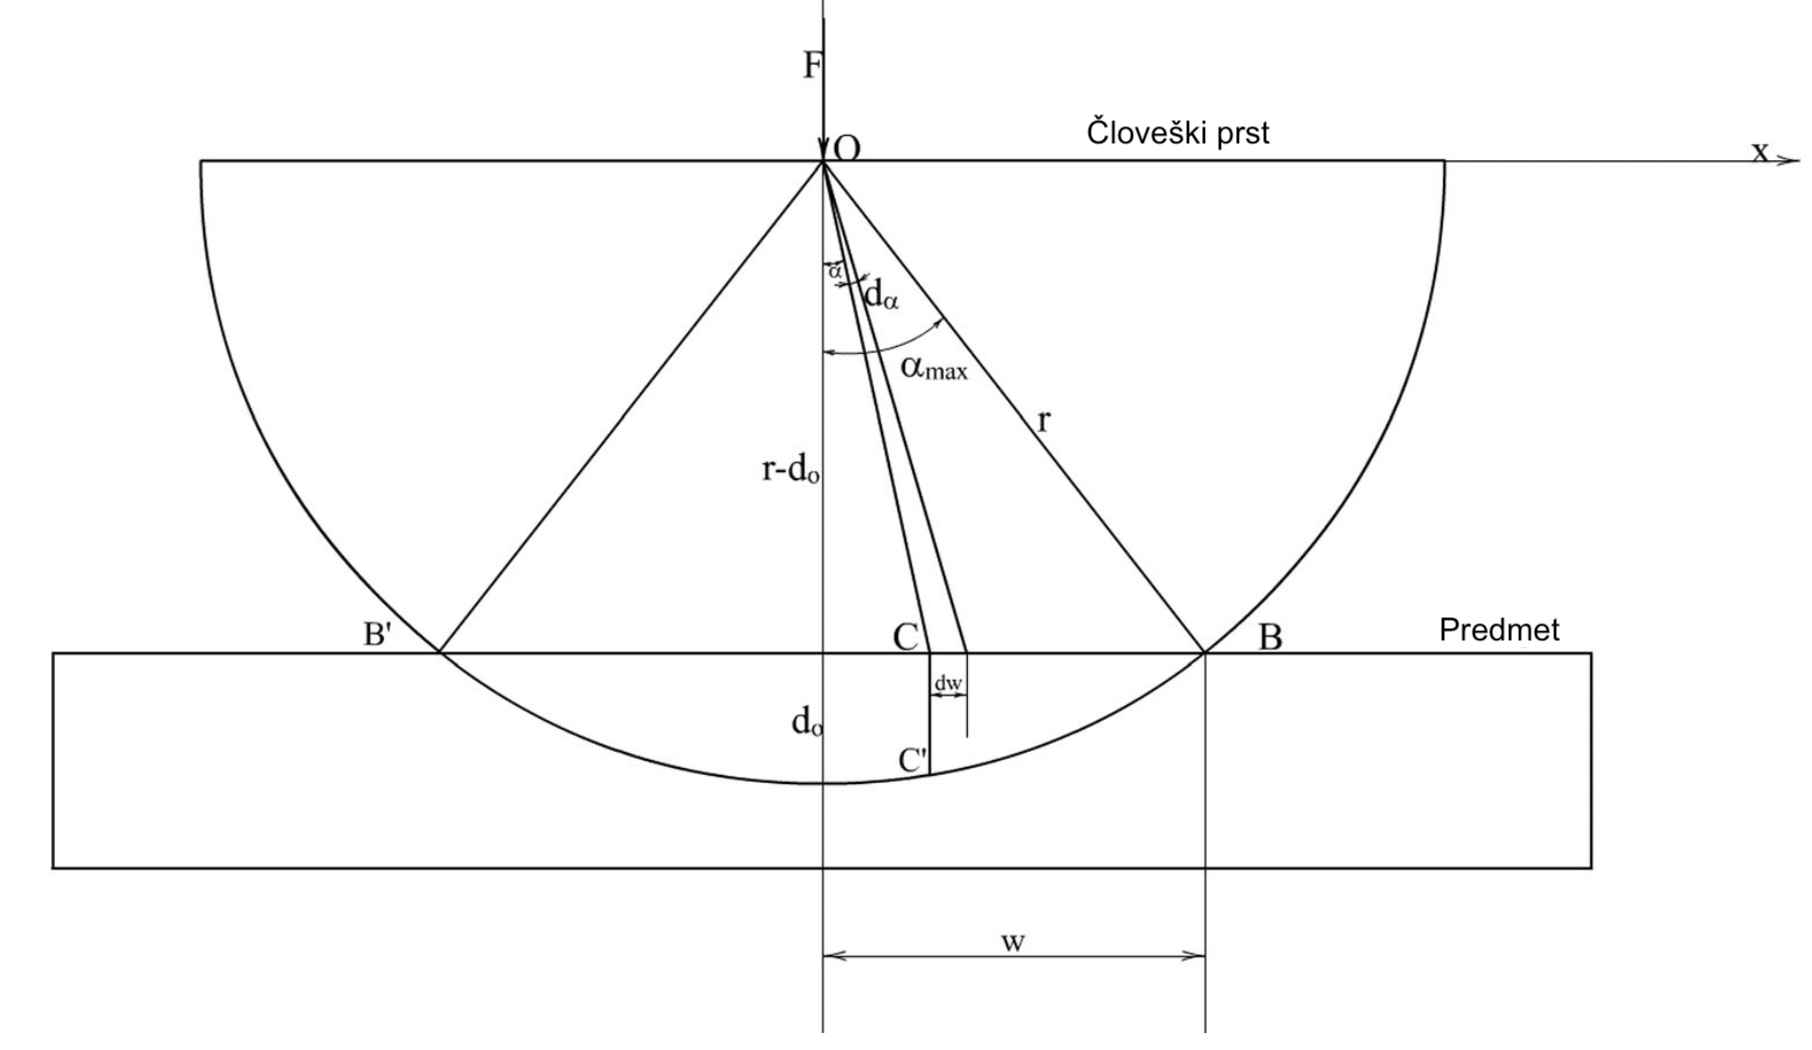
\includegraphics[width=0.8\linewidth]{Screenshot 2026-02-26 at 17.51.56.png}
    \caption{\centering Prečni presek modela prsta, ki se dotika pravokotne površine. Prst si predstavljamo kot polovico valja s polmerom r.}
    \label{prst}
\end{figure}

Najprej kontaktno širino zapišemo s pomočjo kota $\alpha_{max}$ kot $w=(r-d_0)\tan\alpha_{max}.$ Od tu lahko izrazimo $dw$ kot $dw=(r-d_0)/\cos^2\alpha d\alpha.$ Nazadnje zapišemo majhno spremembo kontaktne površine kot $dS=ldw.$

Ko na prst delujemo z kontaktno silo, se polmer prsta vzdolž osi $y$ zmanjša na račun povečanja kontaktne širine. Definiramo kompresijsko obremenitev kot razmerje spremembe polmera in originalnega polmera, $\varepsilon=\Delta r/r=d_0/r.$ Osna napetost, ki deluje na prst, je potem $\sigma=\varepsilon E,$ kjer je $E$ elastični modul. Pri tem uporabimo linearen model deformacije. Končno lahko izračunamo kontaktno silo kot 
\begin{equation}
    \begin{split}
    F_c&=\int_S\sigma dS=El\frac{d_0(r-d_0)}{r}\int_0^{\alpha_{max}}\frac{d\alpha}{\cos^2\alpha}=El\frac{d_0(r-d_0)}{r}\tan\alpha_{max}=\\&=El\frac{d_0(r-d_0)}{r}\frac{w}{r-d_0}=E\frac{d_0wl}{r}.
\end{split}
\end{equation}
Od tu vidimo, da je kontaktna sila odvisna od elastičnega modula, deformacije, kontaktne širine, polmera in dolžine prsta\cite{elango2011analysis}.

\section{Kako delujejo mehki roboti?}
Aktuatorji so umetne mišice, ki mehkim robotom omogočajo premikanje ali deformacije. V nadaljevanju si bomo pogledali nekaj načinov, kako delujejo nekateri izmed najbolj obetavnih aktuatorjev-tekočinski, elektrostatski, elektro-kemični, termalni in magnetni. 
\subsection{Tekočinski aktuator}
\begin{wrapfigure}{r}{0.5\textwidth}
\centering
    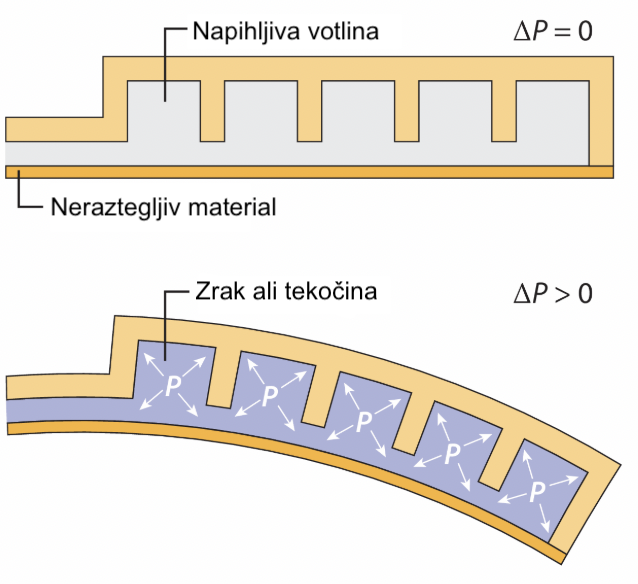
\includegraphics[width=0.48\textwidth]{1_fluidic.png}
  \label{fluidic}
  \caption{Skica premikanja s pomočjo tekočin\cite{yasa2023overview}}
\end{wrapfigure}
Tekočinski aktuator (slika 2) je zelo pogosto uporabljen, saj je izredno preprost. Gibanje doseže s pomočjo polnjenja in praznjenja komor, ki so izdelane iz elastičnega materiala, ena izmed stranic pa je narejena iz neelastičnega materiala. Črpalke črpajo tekočino, kot na primer zrak ali vodo, v komore, ki se zaradi tega raztagnejo, stranica iz neelastičnega materiala pa narekuje, v katero stran se bo aktuator premaknil.

Glavna prednost tekočinskega aktuatorja je, da s spreminjanjem geometrije komor lahko dosežemo zelo široko območje gibanja, ki je lahko upogibanje, ali pa zasuk. Poleg tega za ohranjanje lege ne potrebujemo trošiti dodatne moči, ker lahko zapremo ventil na črpalki.

Glavne slabosti tekočinskega aktuatorja so, da ni odporen na poškodbe, ker začne puščati. Poleg tega zaradi nelinearnega odziva elastične snovi ne moremo doseči velike natančnosti\cite{yasa2023overview}.

\begin{wrapfigure}{r}{0.5\textwidth}
    \centering
    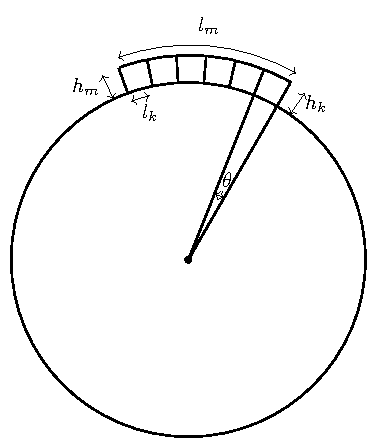
\includegraphics[width=0.48\textwidth]{skica_ukrivljenost.pdf}
  \label{skica}
  \caption{Skica izračuna ukrivljenosti}
\end{wrapfigure}
Poglejmo si, kako izračunamo ukrivljenost takega aktuatorja. V komore višine $h_k$ in dolžine $l_k$ vbrizgamo zrak ali tekočino s tlakom $p.$ Tlak ustvari osno napetost $\sigma_x=p\frac{h_k}{h_m-h_k},$ kjer je $h_m$ višina materiala. Skupna obremenitev $\varepsilon_x$ je nelinearna funkcija osne napetosti, $\varepsilon_x=\varepsilon_x(\sigma_x)$. Za upogib dobimo enačbo $\tan\theta/2=l_k\varepsilon_x(\sigma_x)/(2h_k),$ kjer je $\theta$ kot upogiba. Ker pa imamo $n$ komor, moramo za končen rezultat to pomnožiti s faktorjem $n.$ Od tu lahko izrazimo ukrivljenost aktuatorja kot $$\kappa=\frac{\theta}{l_m}=\frac{2n}{l_m}\arctan\frac{l_k\varepsilon_x(\sigma_x)}{2h_k},$$ kjer je $n$ število komor (razdelkov) in $l_m$ dolžina materiala\cite{onal2013autonomous}.
\\ \\ \\
\subsection{Elektrostatični in elektrokemični aktuator}
Elektrostatično in elektrokemično aktiviranje se zgodi z neposrednim pretvarjanjem električne energije v deformacijo mehkega telesa (in toploto). Na ta princip deluje več različnih vrst aktuatorjev. V osnovi so vsi aktuatorji tega tipa podobni kondenzatorju: sestavljeni so iz dveh plošč, ki jih nabijemo; ter dielektričnega sredstva v sredini.
\begin{wrapfigure}{r}{0.5\textwidth}
\centering
    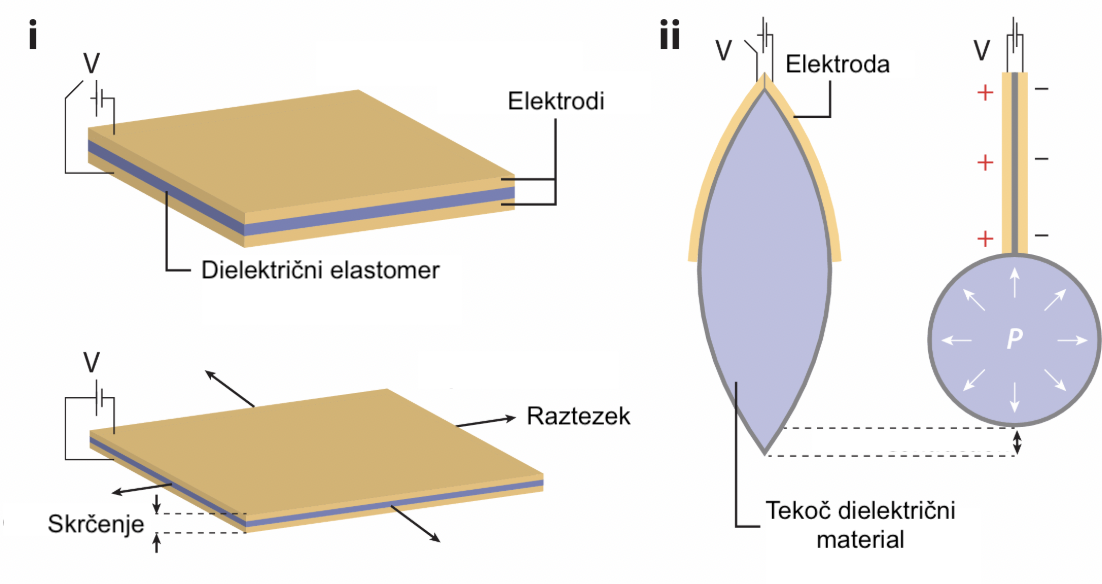
\includegraphics[width=0.48\textwidth]{2_electrostatic.png}
  \label{2}
  \caption{Skica premikanja s pomočjo dielektričnega elastomera(i) ter tekočega dielektrika(ii)\cite{yasa2023overview}}
\end{wrapfigure}
\subsubsection{Elektrostatični aktuatorji} 
Kot je prikazano na sliki 4(i), je aktuator iz dielektričnega elastomera sestavljen iz dveh elastičnih prevodnih plošč, med njima pa je dielektrično sredstvo. Ko na plošči priključimo napetost, se razdalja med ploščama zmanjša zaradi električne sile; plošči pa se raztegneta. Glede na postavitev se sistem lahko raztegne, skrči ali zasuka.

Hidravlični elektrostatski aktuator (slika 4(ii)) je ponavadi narejen tako, da elastično telo, napolnjeno z dielektrično tekočino (npr. olja), delno obdamo z elektrodami. Ko nanj priključimo napetost, pride do velikega raztega v delu brez elektrod. Sistem se obnaša podobno kot mišice.

Elektrostatični aktuatorji so zelo uporabni, saj obstaja direktna povezava med napetostjo med ploščama ter raztegom, zato lahko z njim dosegamo zelo dobro natančnost.

Slabost tega načina je, da potrebuje kar velike napetosti ($0.3-27$kV), poleg tega se sistem ob izklopu napetosti vrne v osnovno stanje\cite{yasa2023overview}.
\begin{wrapfigure}{r}{0.5\textwidth}
\centering
    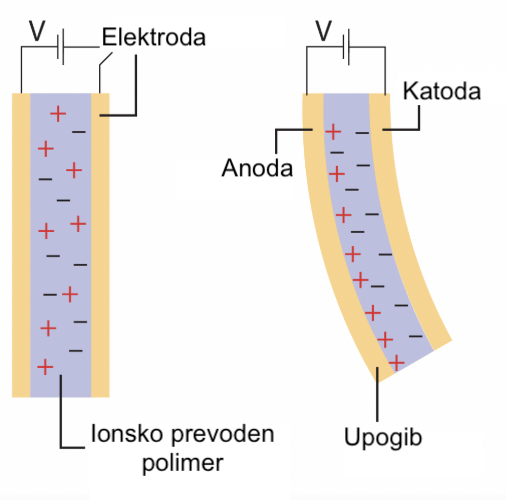
\includegraphics[width=0.48\textwidth]{3_electrochemical.png}
  \label{3}
  \caption{Skica elektrokemičnega aktuatorja: ko nanj priključimo napetost, se kationi pomaknejo proti anodi, polimer pa se ukrivi\cite{yasa2023overview}}
\end{wrapfigure}
\subsubsection{Elektrokemični aktuatorji}
Elektrokemični aktuatorji so sestavljeni iz ionsko prevodnega polimera, obdanega z dvema vzporednima elastičnima elektrodama. V polimeru se anioni ne premikajo, kationi pa so prosti. Ko na elektrodi priključimo napetost, se kationi v polimeru prerazporedijo in povzročijo, da se sistem upogne.

Glavna prednost tega sistema je, da lahko natančno nadziramo upogib, poleg tega pa sistem za razliko od elektrostatičnih aktuatorjev potrebuje precej manjšo napetost ($1-5$V).

Slabost sistema je, da se premikanje odvija precej počasi, saj je odvisno od hitrosti premikanja kationov v polimeru. Poleg tega pa mora biti polimer precej navlažen, zato sistem potrebuje vlažno okolje, da sploh lahko deluje, kar predstavlja problem za elektroniko.

\begin{wrapfigure}{r}{0.5\textwidth}
\centering
    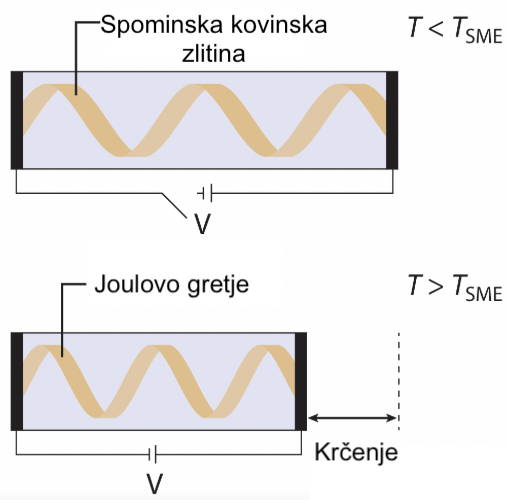
\includegraphics[width=0.48\textwidth]{4_thermal.png}
  \label{4}
  \caption{Skica termičnega aktuatorja\cite{yasa2023overview}}
\end{wrapfigure}
\subsection{Termični aktuator}
Za termične aktuatorje se najpogosteje uporablja spominske kovinske zlitine (shape memory alloys). Če deformirano zlitino segrejemo, kar najlažje naredimo s tem, da nanjo priključimo napetost, se ta vrne nazaj v začetno stanje zaradi Joulovega gretja. Ko se zlitina spet ohladi, se ne vrne v deformirano stanje.

Spominske zlitine so v ravni obliki zmožne doseči malo pod 10\% raztezka, če pa jih oblikujemo v spiralo, pa lahko dosežemo tudi do 300\% raztezka.

Največja slabost termičnih aktuatorjev je njihova odvisnost od temperature, kar močno poslabša njihovo učinkovitost. Poleg tega je njihovo premikanje precej počasno\cite{yasa2023overview}.\\ \\

\begin{wrapfigure}{r}{0.5\textwidth}
\centering
    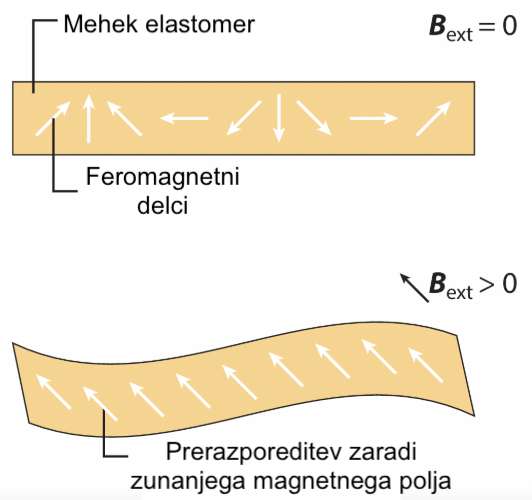
\includegraphics[width=0.48\textwidth]{5_magnetic.png}
  \label{5}
  \caption{Skica magnetnega aktuatorja\cite{yasa2023overview}}
\end{wrapfigure}
\subsection{Magnetni aktuator}
Magnetni aktuatorji so sestavljeni iz mikroskopskih feromagnetnih delcev, ujetih v mehkem elastomeru. Ko strukturo postavimo v zunanje magnetno polje, se feromagnetni delci uredijo v željeno strukturo. 

Aktuatorji te vrste so izredno uporabni za operacije na živih bitjih, saj jih lahko premikamo po ceveh (na primer žilah), ne da bi pri tem ogrozili osebo.

Po drugi strani pa potrebujemo za premikanje aktuatorjev precej močne permanentne magnete, prav tako pa so zelo občutljivi na ostale megnete ter kovinske materiale v bližini\cite{yasa2023overview}.\\ \\ \\ \\

\section{Robotska hobotnica}
Za konec si poglejmo še primer robota, ki so ga ustvarili po zgledu hobotnice. Hobotnica predstavlja navdih za mehke robote predvsem zato, ker nima v telesu nobene kosti, proti čemur težijo tudi mehki roboti, ki so sestavljeni predvsem iz mehkih materialov. Poleg tega je hobotnica sposobna svoje telo močno deformirati in prilagoditi okolju.

\textbf{Opomba}: hobotnica, ki jo obravnavamo, ni povsem mehek robot, temveč je hibrid, ampak se bomo v nadaljevanju osredotočili na dele, ki upoštevajo spoznanja mehke robotike.
\begin{figure}[h]
    \centering
    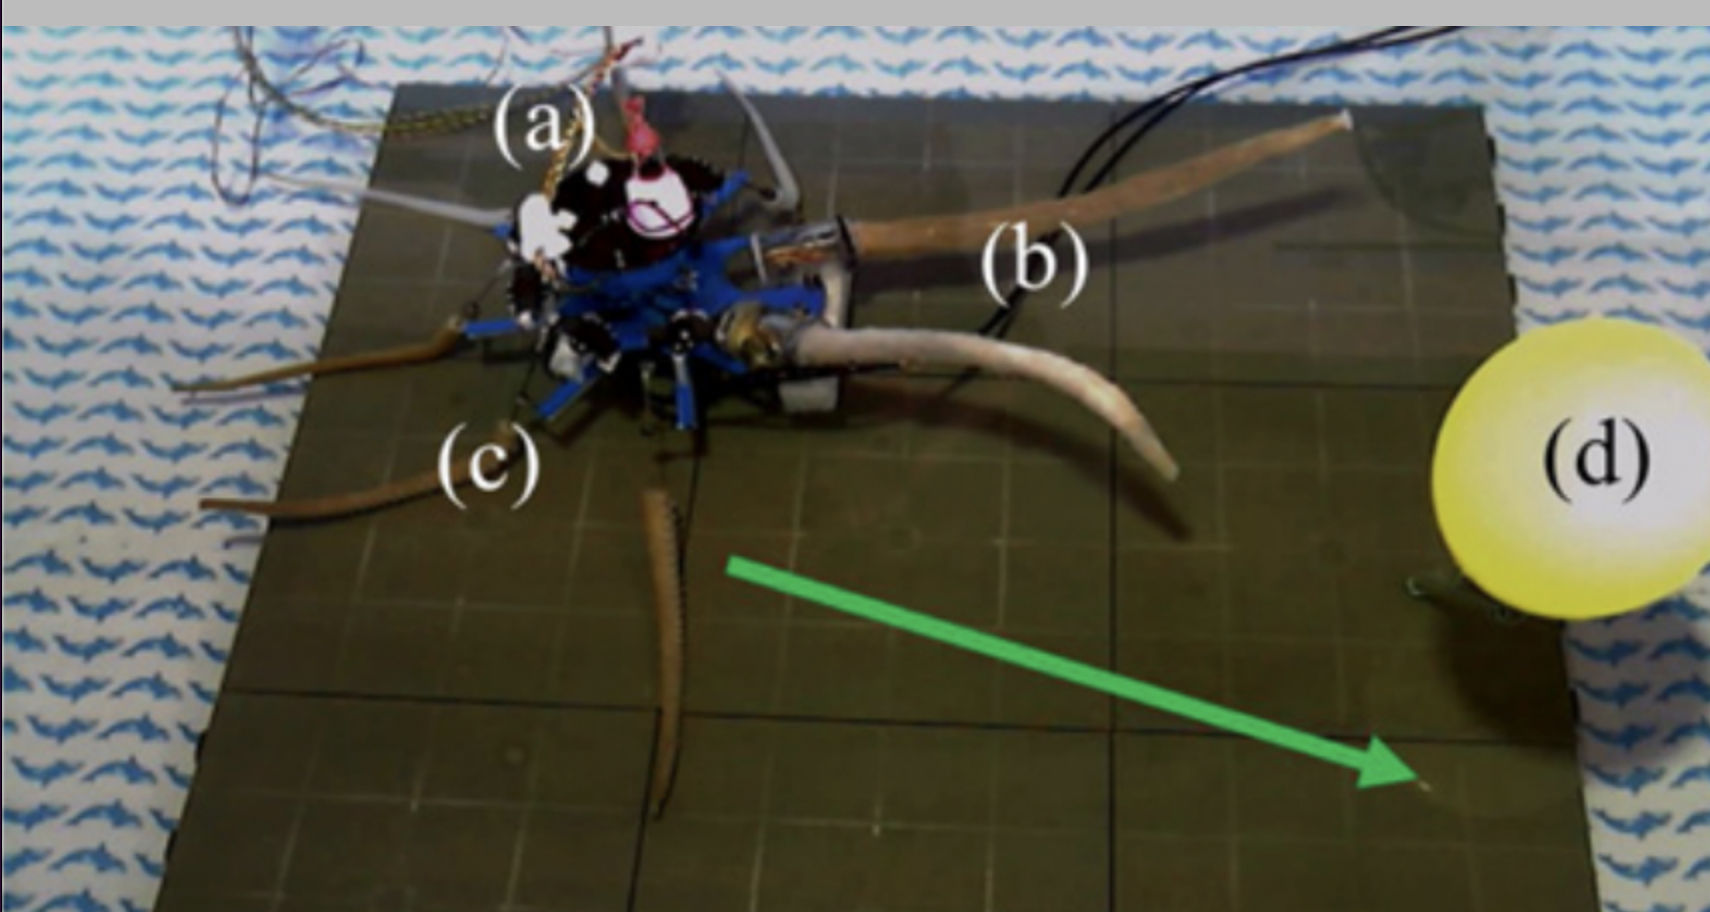
\includegraphics[width=0.5\linewidth]{hobotnica.png}
    \caption{Robotska hobotnica\cite{cianchetti2015bioinspired}}
    \label{hobo}
\end{figure}

\noindent Na sliki 8 je prikazana robotska hobotnica. Z (a) je označen osrednji del s kamero; z (b) sta označeni roki, namenjeni manipulaciji z objekti; s (c) so označene roke, ki premikajo hobotnico; z (d) pa balon-tarča, proti kateri se robot premika. Vsa elektronika je spravljena v osrednjem delu s kamero.

Sprednji roki, namenjeni za manipulacijo, sta se sposobni podaljšati, skrajšati, upogniti v katerokoli smer in spreminjati svojo trdoto. Sestavljeni sta iz vzmeti iz spominskih kovinskih zlitin in aktuatorjev z motorji. Za prenos gibanja iz aktuatorjev na ostale dele roke poskrbijo pletene niti iz polietilena. Lovki sta obdani s plastjo umetne kože, debele manj kot 1mm.

Preostalih 6 rok je sestavljenih iz silikona, ki obdaja jekleno žico. Ko potegnemo žico, se roka upogne v željeno smer. Pri premikanju večina rok drži robota na določeni višini nad podlago, preostale roke pa z upogibanjem dosežejo premik.

Robotska hobotnica je eden izmed prvih mehkih robotov, ki je sposoben premikanja in manipulacije z objekti. Vključuje kar nekaj spoznanj, ki smo jih opazili pri gibanju hobotnice, kot na primer način premikanja\cite{cianchetti2015bioinspired}.

\section{Zaključek}
Mehka robotika predstavlja sodobno in hitro razvijajoče se področje, ki temelji na uporabi mehkih, deformabilnih materialov namesto klasičnih togih struktur. V nasprotju s tradicionalno robotiko, kjer gibanje izhaja iz diskretnih členov in sklepov, mehki roboti svoje funkcije dosegajo preko zveznih deformacij, ki jih opisujemo z zakonitostmi kontinuumske mehanike.

Kljub hitremu napredku ostajajo odprti številni problemi, predvsem na področju modeliranja velikih deformacij, nadzora kontinuumskih sistemov ter razvoja novih funkcionalnih materialov. Mehka robotika tako predstavlja izrazito interdisciplinarno področje, kjer se prepletajo fizika mehke snovi, materialna znanost in inženirstvo.

V prihodnosti lahko pričakujemo, da bo boljše razumevanje fizikalnih principov mehkih materialov omogočilo razvoj naprednejših, prilagodljivih in varnih robotskih sistemov, ki bodo našli uporabo v medicini, industriji in interakciji z ljudmi.

\newpage
\printbibliography

\end{document}
